This chapter will first introduce PyNN, an high level language based on Python used to implement spiking neural networks, and then will describe the network in detail.

\section{PyNN}
PyNN is a Python library which defines a high level interface to create spiking neural networks in a simulator-agnostic fashion \cite{Davison2008}. Once a network is defined using PyNN, it can then be run on several available simulators, like NEST, NEURON and Brian, and different neuromorphic platforms, like SpiNNaker. In order to run PyNN scripts on SpiNNaker, sPyNNaker has been developed by the SpiNNaker group at the University of Manchester \cite{Rhodes2018}.

\begin{figure}[ht]
\centering
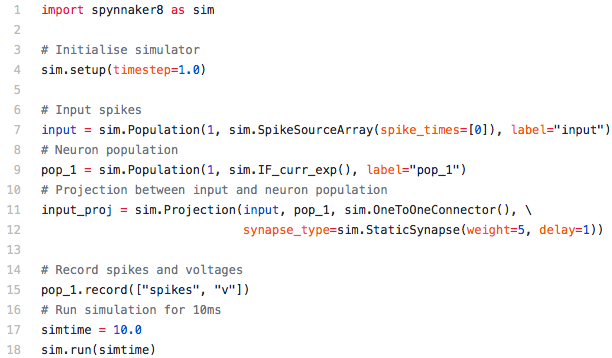
\includegraphics[scale=0.5]{images/development/pynn_example.png}
\caption[PyNN Example]{PyNN code example.}
\label{fig:pynn_example}
\end{figure}

PyNN defines spiking neural networks in terms of neurons grouped together in \emph{populations}. These populations are linked together using \emph{projections}. These projections use connection algorithms which can be selected from built-in methods or be explicitly defined. Parameters of the populations, like spike trains or voltages, can be recorded during the simulation and can be accessed when it is completed for further analysis. A brief code example is provided in \cref{fig:pynn_example}. 

\section{Shape Tracking Spiking Neural Network}
The network developed for this project draws its inspiration from the HMAX model proposed by Riesenhuber and Poggio \cite{Riesenhuber1999}. This model builds a hierarchy of increasingly complex representation in order to perform edge detection. An overview is shown in \cref{fig:hmax}. The \textsc{S1} and \textsc{C1} cells are part of the primary visual cortex V1.  

\begin{figure}[ht]
\centering
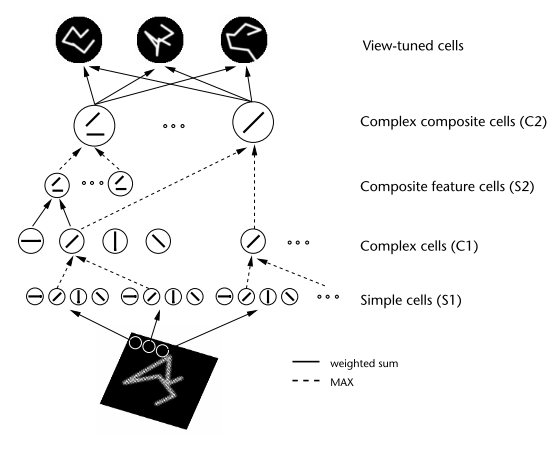
\includegraphics[scale=0.5]{images/development/hmax.png}
\caption[HMAX Model]{The HMAX model by Riesenhuber and Poggio \cite{Riesenhuber1999}.}
\label{fig:hmax}
\end{figure}

This model carries out edge detection alternating two main types of cells: simple cells \textsc{S} performing Gaussian-like tuning operations and complex cells \textsc{C} performing max operations. The \textsc{S} cells are of particular interest: they act as simple edge detector for the 4 main orientation of a line (horizontal, vertical, right diagonal and left diagonal) and they can be combined in order to obtain a desired shape. The \textsc{C} cells, with their max operation provide translation invariance and they are not useful for tracking shapes moving in a video stream.

Based on these ideas, the network used in this project had been designed. A diagram is provided in \cref{fig:network}. The network is composed of 8 neuron populations, each comprising  $32 \times 32 = 1024$ LIF neurons, divided in 3 ``layers'': the DVS outputs, the receptive fields and the shapes detectors. The input of the DVS has a spatial of resolution $32 \times 32$ pixels and it could be either a prerecorded video or a live recording using a webcam. Keeping all populations of size $32 \times 32$ allows the neurons to have a one-to-one mapping with the pixels in the input video stream. 

\begin{figure}[ht]
\centering
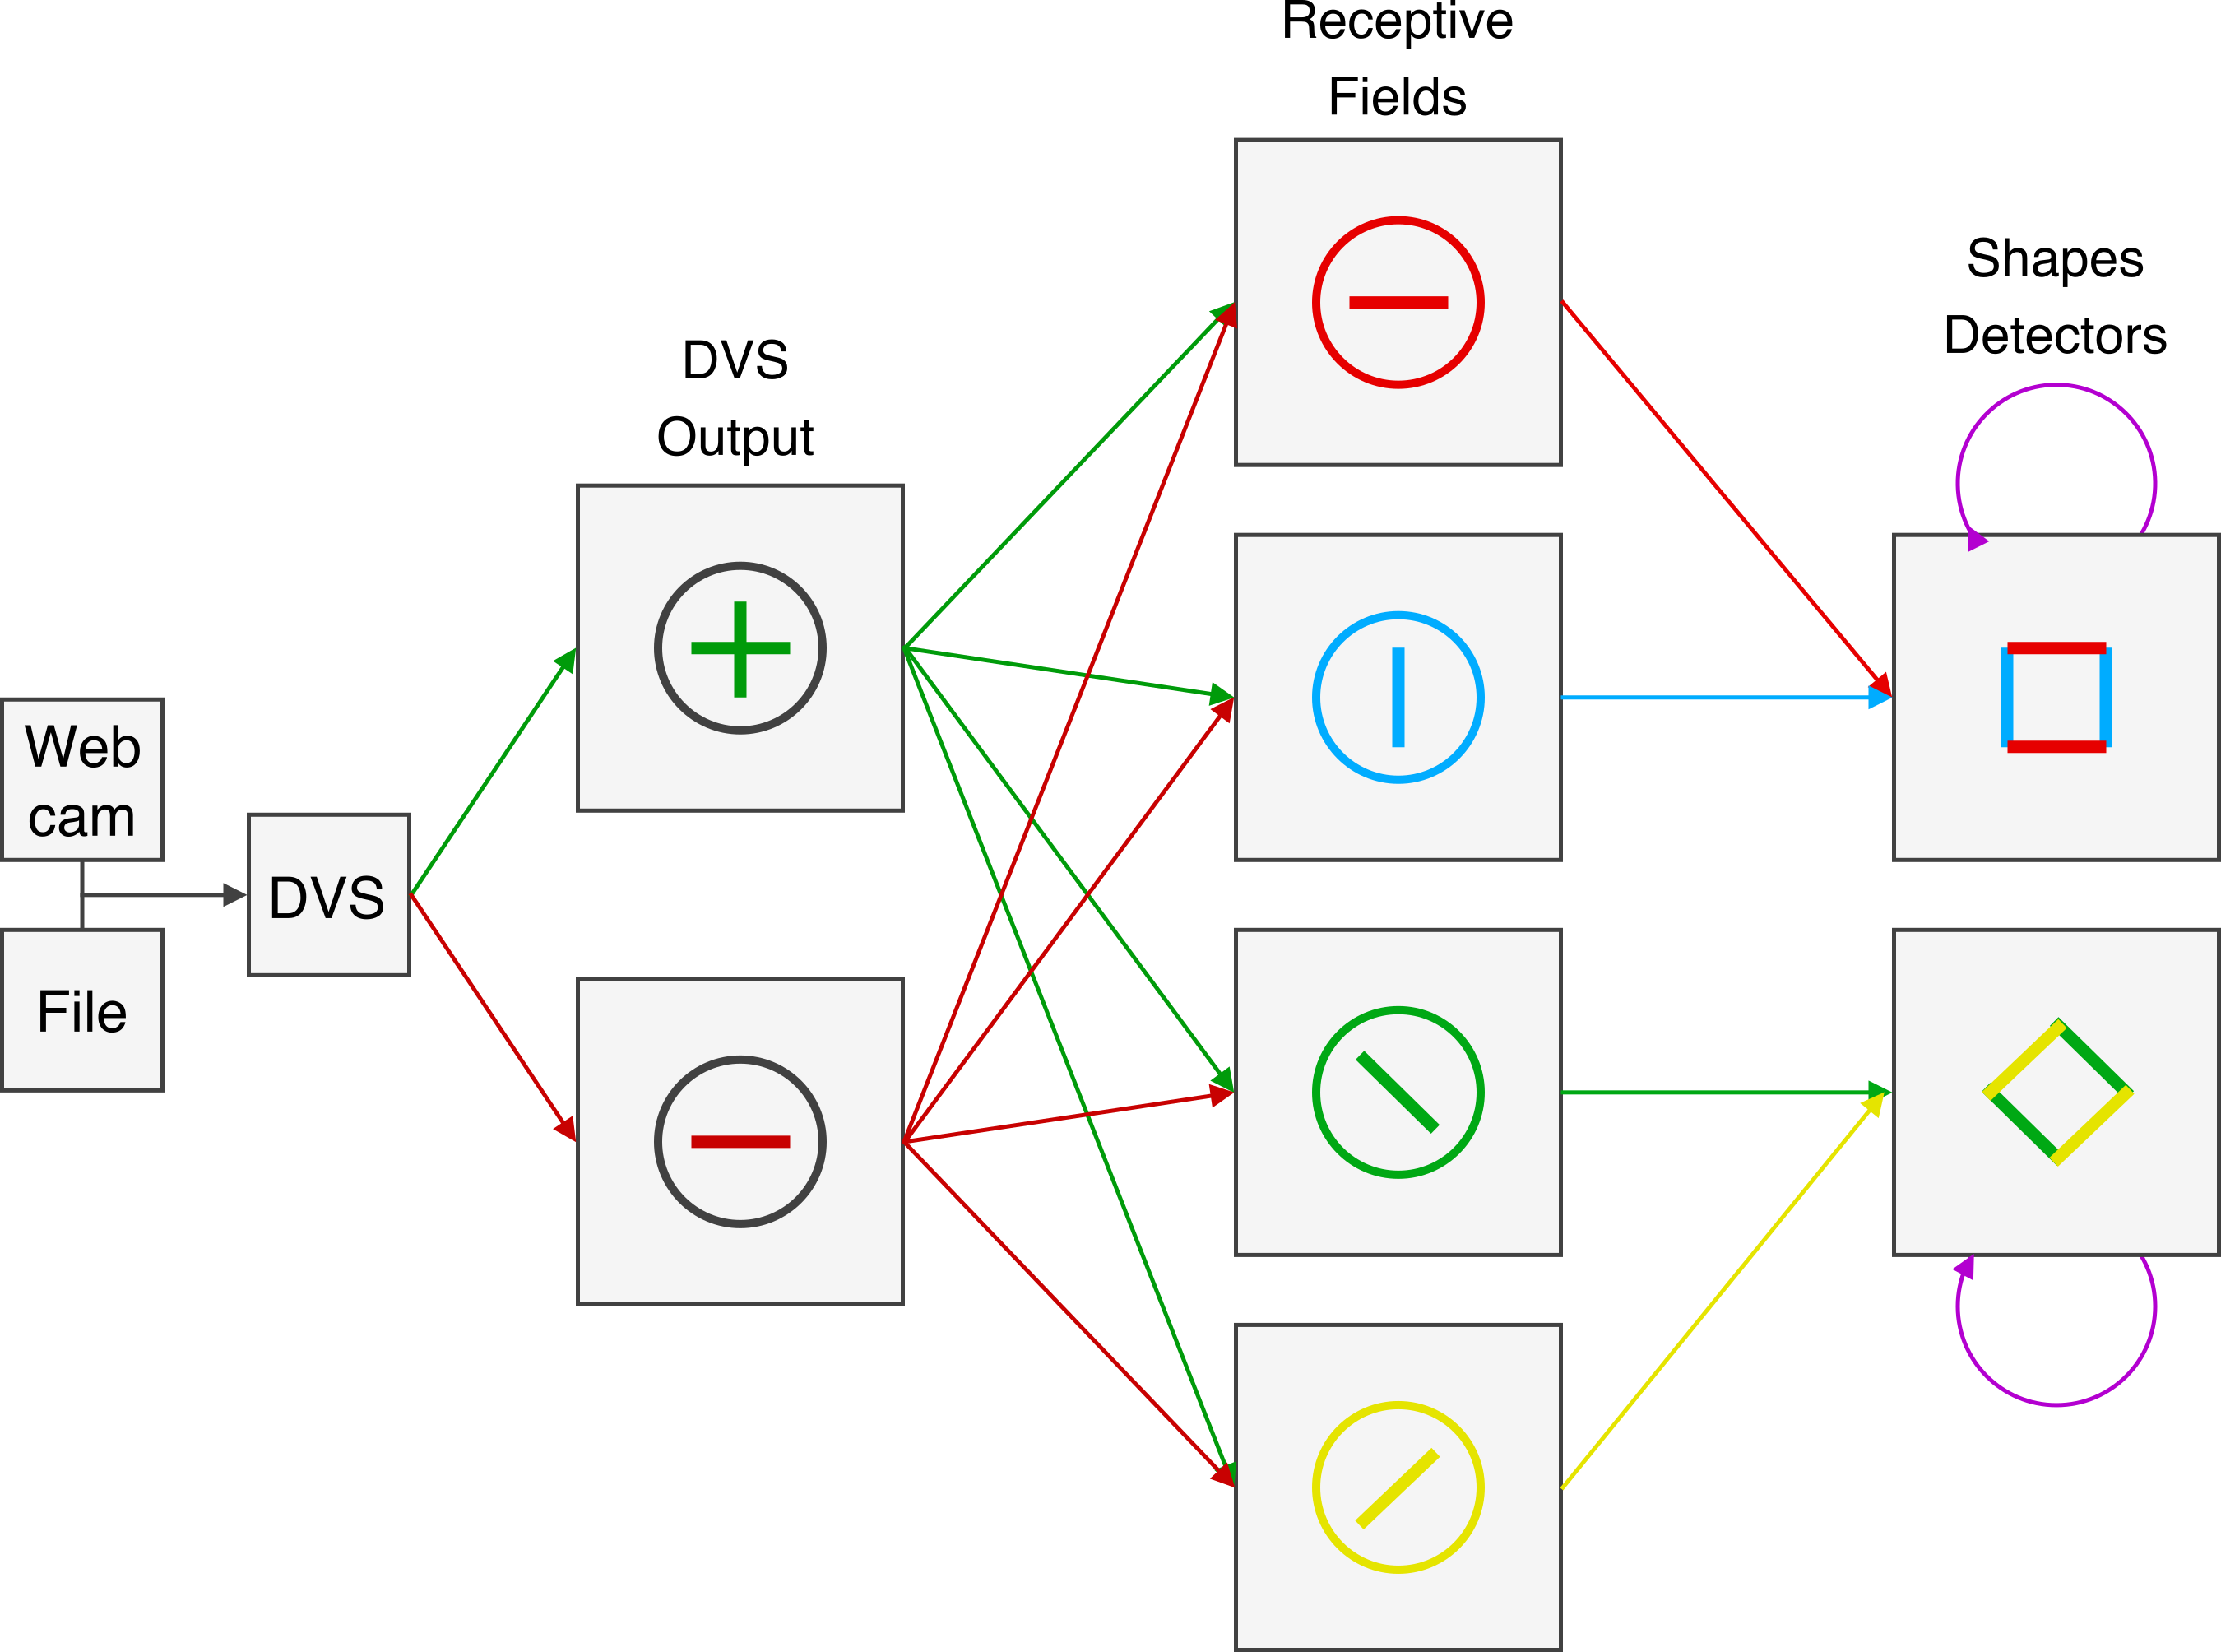
\includegraphics[width=0.75\textwidth]{images/development/network.png}
\caption[Network Overview]{The network developed for this project. The squares represent neuron populations, the arrows are the connections between populations.}
\label{fig:network}
\end{figure}


\subsection{DVS Emulator Output}
The DVS emulator produces two separate spikes streams, one for positive changes in pixel brightness (the green ones in \cref{fig:network}) and one for negative ones (the red ones). These spikes are injected into the network using two \texttt{SpikeSourceArray}, a PyNN object which emits spikes at specific times and can be treated in a similar way to a normal neuron population. The input of a \texttt{SpikeSourceArray} is a list of times for each neuron in the population. 

\begin{figure}[ht]
\centering
\subcaptionbox{Screenshot of a video of a white square moving on a black background from left to right. \label{fig:dvs_square_lr}}
  [0.47\textwidth]{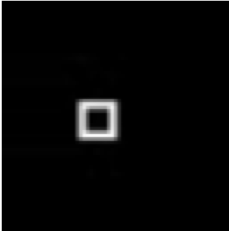
\includegraphics[width=0.30\textwidth]{images/development/dvs_square_lr.png}}
\subcaptionbox{DVS output of the same square moving from left to right. In yellow the positive spikes and in purple the negative ones. \label{fig:spikes_square_lr}}
  [0.47\textwidth]{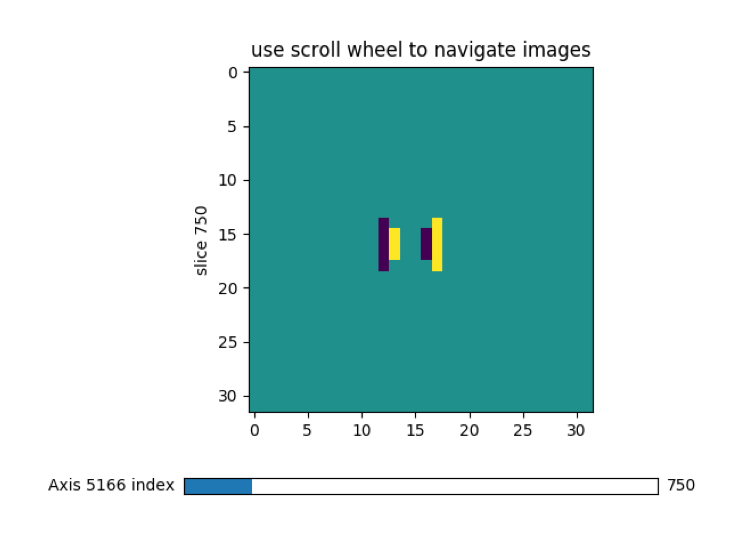
\includegraphics[width=0.4\textwidth]{images/development/spikes_square_lr.png}}
\caption[DVS Output of a Square]{Screenshot and DVS output of a square moving from left to right on the screen.}
\label{fig:square_lr}
\end{figure}

In \cref{fig:square_lr}, a \SI{5}{s} video of a white square moving from left to right is shown. This video has been synthetically generated using a Python script. The DVS emits spikes only on the horizontal edges and on the first pixel of the top and bottom edges. This is due to the fact that on the top edge (and the bottom one), the pixel brightness does not change, apart from the rightmost and leftmost pixels.

\subsection{Receptive Fields}
In the context of the visual system, a receptive field is a region of the retina associated with a neuron which spikes when the region is stimulated by light. The neurons in this layer are the \textsc{S1} cells discussed previously. These form 4 populations of cells, one for each of the 4 bar orientations (horizontal, vertical and the two diagonals). 

The receptive fields are modelled upon the Octopus retina, as described by Folowosele in \cite{Folowosele2011}. An illustration is provided in \cref{fig:receptive_fields}.

\begin{figure}[ht]
\centering
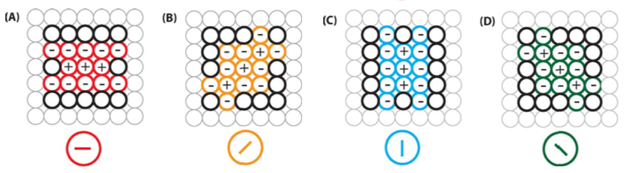
\includegraphics[scale=0.6]{images/development/receptive_fields.png}
\caption[Receptive Fields]{Illustration of the receptive fields of the \textsc{S1} cells implemented in the network. The $+$ represents excitatory connections, the $-$ represents inhibitory connections and the empty circles have no effects on \textsc{S1} cells.}
\label{fig:receptive_fields}
\end{figure}

The receptive fields are constructed using connections between the positive and negative polarities \texttt{SpikeSourceArray}s, the DVS output layer in \cref{fig:network}, and the 4 populations of \textsc{S1} cells. Each neuron in a \textsc{S1} cells population has 3 excitatory connections to the positive polarity \texttt{SpikeSourceArray} and 10 inhibitory connections to the negative polarity \texttt{SpikeSourceArray} accordingly to the patterns shown in \cref{fig:receptive_fields}. For neurons close to the edges, only the connections falling inside the $32 \times 32$ frame are set.

An example of the behaviour of these populations of cells is shown in \cref{fig:receptive_fields_square_lr}.

\begin{figure}[ht]
\centering
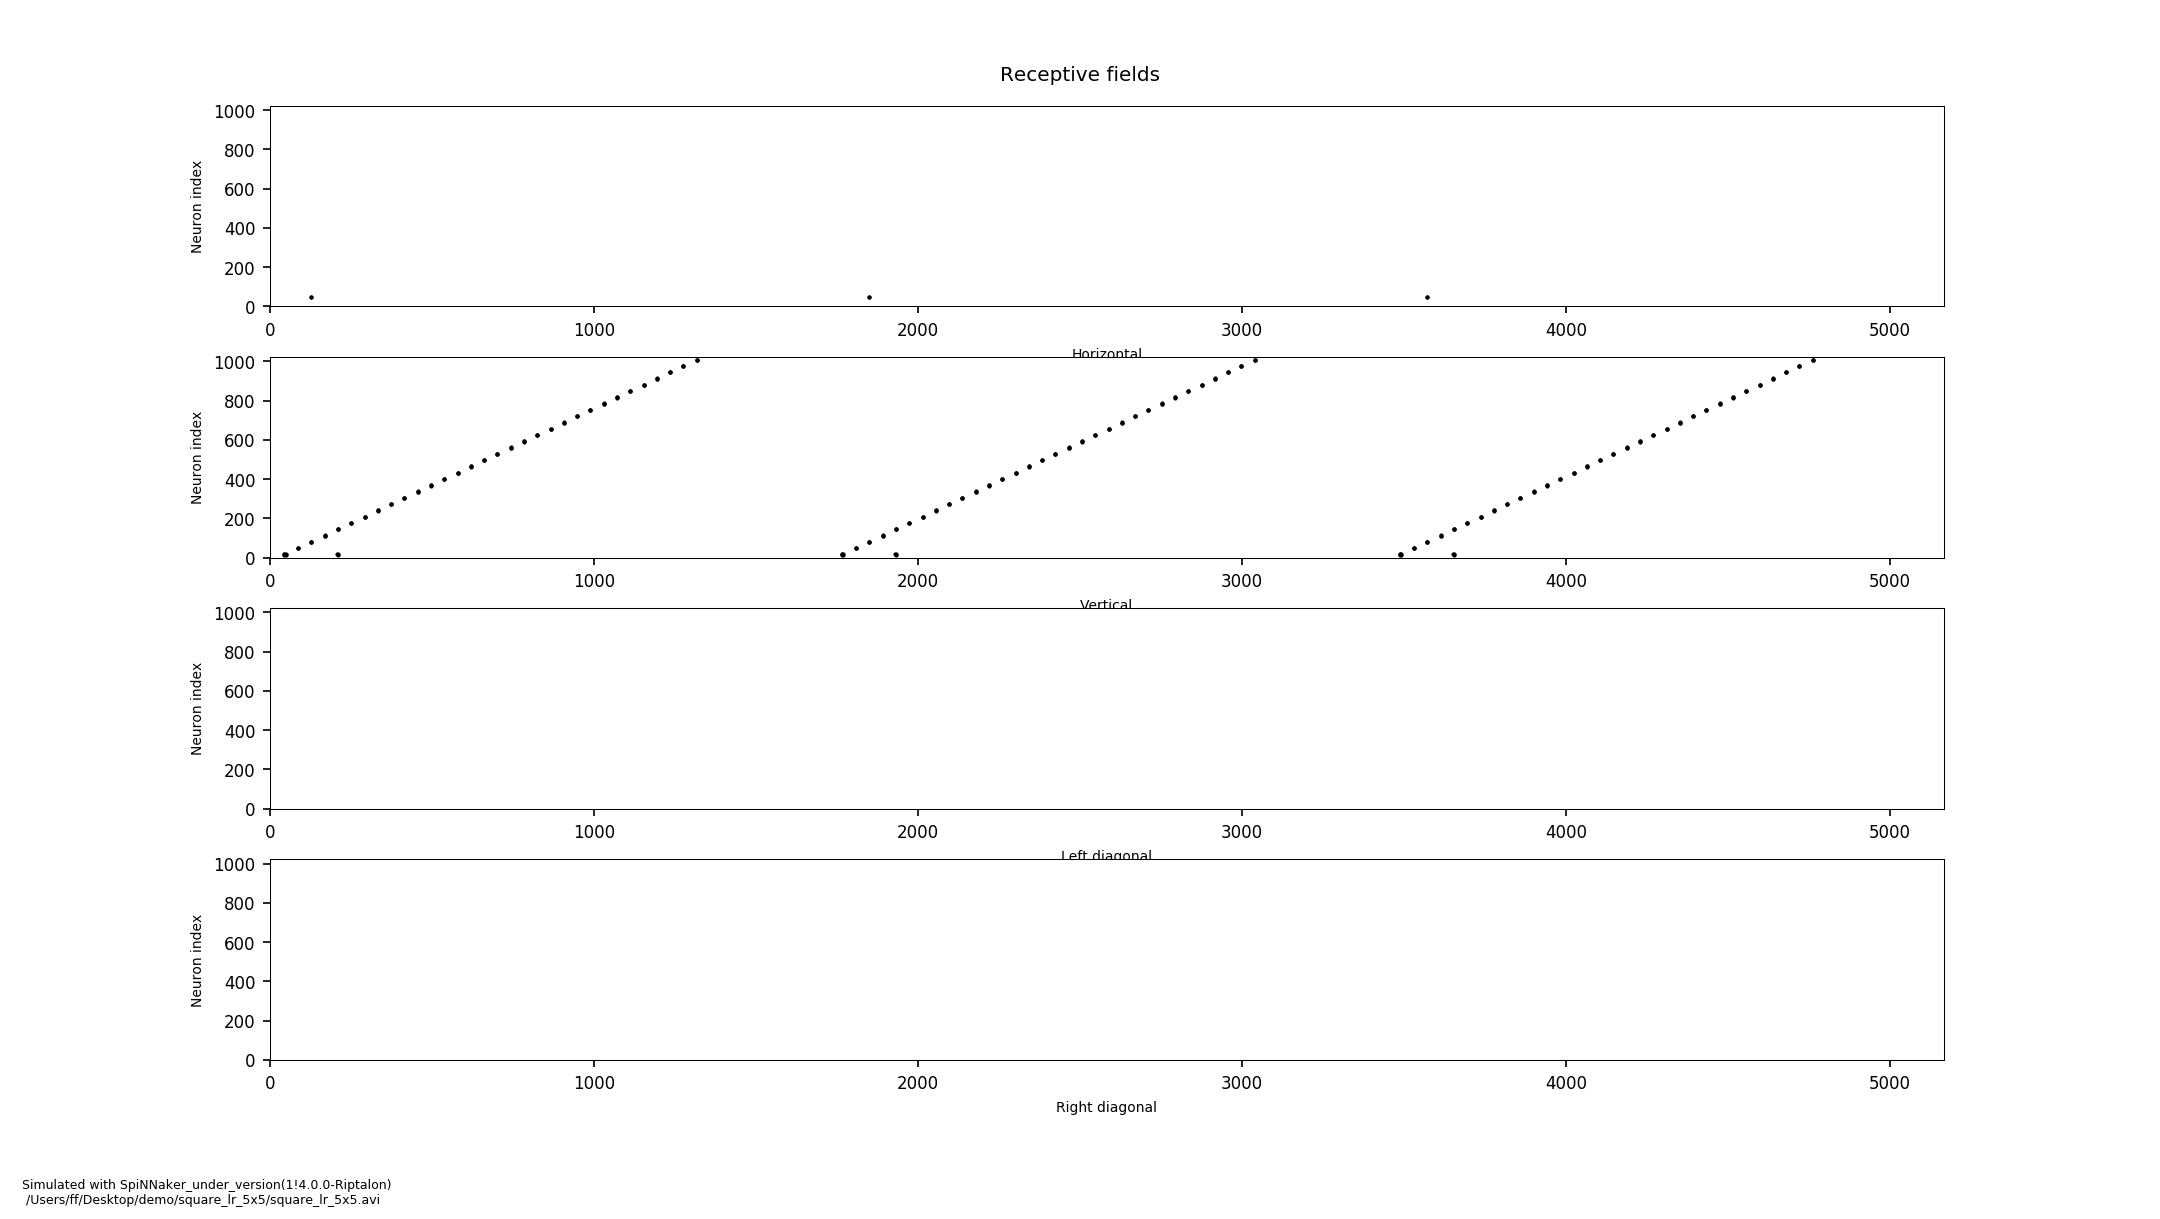
\includegraphics[width=\textwidth]{images/development/receptive_fields_square_lr.png}
\caption[Receptive Fields Spike Trains of Square]{Spike trains of the 4 population of cells when the video of the square moving from left to right is presented. From top to bottom: horizontal, vertical, left diagonal (green in \cref{fig:receptive_fields}) and right diagonal (yellow in \cref{fig:receptive_fields}). On the $x$ axis there is time in milliseconds, on the $y$ axis the neuron ids. In this example it can be seen that only vertical edges are found and some small noise on the horizontal ones due to the square entering the screen. Due to resolution constraints not all the spikes can be seen, a single dot comprises multiple spikes.}
\label{fig:receptive_fields_square_lr}
\end{figure}

\subsection{Shapes Detector}
Once the receptive fields had been set up, they can be combined in various ways, in order to create populations of cells able to detect shapes.

The network in its current form recognises only two shapes: a square and a diamond. For each shape, a population of cells had been created.

The ``square detector'' combines horizontal and vertical edges in order to detect squares of size $5 \times 5$. On the other hand, the ``diamond detector'' combines the left and right diagonal edges to detect diamonds of size $5 \times 5$. 

The connections between the \textsc{S1} cells populations and the shapes detectors are all excitatory. In this way, the neuron which spikes in the shape detector population is at the centre of the location of the shape in the visual plane. 

This setup has one obvious disadvantage: it does not account for scale variance. In order to account for it, connections to the surrounding cells are added. An example of this, for the vertical edges of the square detector, can be seen in \cref{fig:shapes_connections}. The other edges behave in a similar way. With this technique, shapes of size 3, 5, 7 and 9 are accounted for. 

\begin{figure}[ht]
\centering
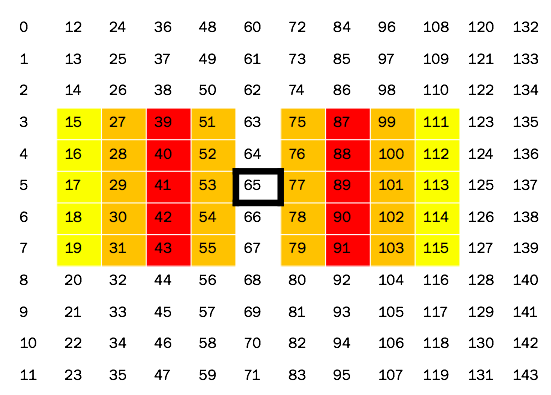
\includegraphics[width=0.75\textwidth]{images/development/shapes_connections.png}
\caption[Vertical Edges of the Square Detector]{For this example, a $12 \times 12$ input area is used, where the numbers represents the neuron ids. Neuron 65 in the square population has connections to all the neurons highlighted in the respective edge population, in this case the vertical one. The red connections have the strongest connection weight and the yellow one the weakest.}
\label{fig:shapes_connections}
\end{figure}

Due to the increased number of connections, false positives can occur. In order to reduce them, a biological mechanism called lateral inhibition is used. It is represented by the purple arrows in \cref{fig:network}. With lateral inhibition, an excited neuron will send a inhibitory signal to all the surrounding neuron. Thanks to this mechanism, the first neuron that spikes in the shape population stops the others from spiking.

\subsection{Shape Recognition}
At this point, the spike trains from the shape detector populations can be used to locate and track the shape across time. An example of it is shown in \cref{fig:shape_detectors}. It can be seen that, even with lateral inhibition, multiple neurons spike at the same time. In that case, the marker is arbitrarily selected taking the median of the neuron ids. 

\begin{figure}[ht]
\centering
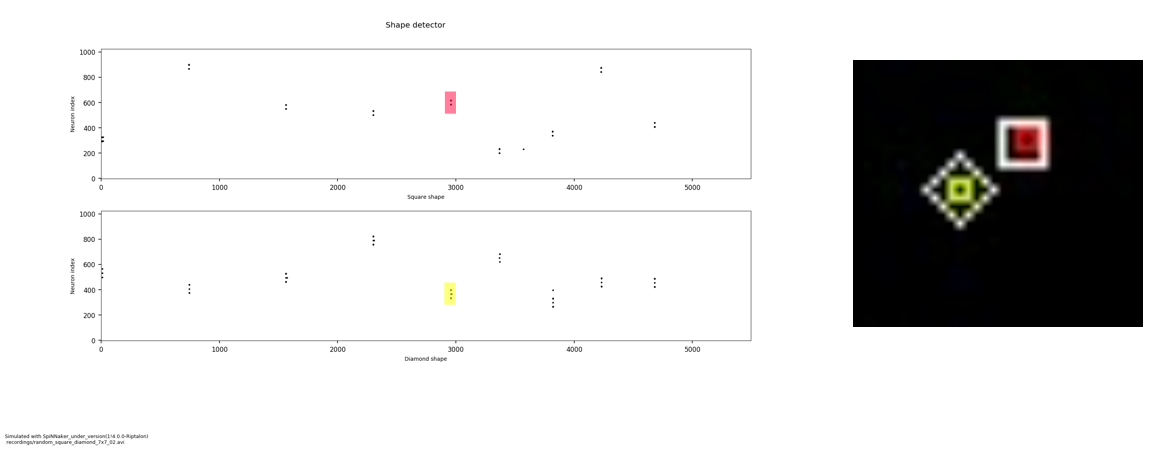
\includegraphics[width=\textwidth]{images/development/shape_detectors.png}
\caption[Shapes Detector with Square and Diamond]{On the left the spike trains for the square (top) and diamond (bottom) populations. On the right a screenshot of the video used as an input at the time highlighted in the spike train, with a yellow marker which tracks the position of the diamond and a red marker for the square. It can be seen how 3 neurons spike in the diamond detector and the selected one (the median) is the correct one. On the other hand, in the square population only 2 neurons spike and the wrong one is selected.}
\label{fig:shape_detectors}
\end{figure}

